\section{Evaluation}
\label{cha:evaluation}

We evaluate our approach through (i)~a proof-of-concept implementation and (ii)~a number of experiments in which we assess performance overheads of \textit{tinyFaaS} and compare it to two alternative approaches from related work.

\subsection{Proof-of-Concept Implementation}
\label{sec:implementation}

As described, \textit{tinyFaaS} comprises three main components: the reverse proxy, the function handlers, and the management service.
For simplicity, in our proof-of-concept, only a Node.js v8 runtime is supported.
The function handlers are Docker containers running a Node.js script with an HTTP endpoint that accepts any incoming requests using the \texttt{http} module.
The actual function code is loaded as a module to that script and its exposed function is executed for each incoming request.

The management service is a Python3 application that uses \texttt{docker-py} to manage the Docker containers, images, and networks needed for \textit{tinyFaaS}.
It exposes an HTTP endpoint for us to add new functions to \textit{tinyFaaS}.
When a new function is created, the management service creates a configurable number of Docker containers that each contains a function handler for the function.
For each function, it also creates a dedicated Docker network to which it attaches all function handlers and the reverse proxy.

We implemented the reverse proxy in Go, using the \texttt{go-coap} library.
The reverse proxy accepts incoming HTTP requests from the management service to create a new CoAP resource with a given identifier and given IP addresses of existing Docker containers on the \textit{tinyFaaS} host that incoming CoAP requests should be forwarded to.
The small binary that the reverse proxy compiles to is then also run in a Docker container.
Our implementation is available as open-source software\footnote{\url{https://github.com/OpenFogStack/tinyFaaS}}.

\subsection{Experiment Setup}
\label{sec:experiment}


In our experiments, we compared \textit{tinyFaaS} to both an existing edge FaaS platform and a high-performance cloud FaaS platform.
We also assessed the \textit{tinyFaaS} overhead by comparing its performance to the performance of a native, non-dockerized Node.js deployment on the same machines.
This native implementation also uses a CoAP endpoint, which should help us understand how the internal design of \textit{tinyFaaS} affects performance rather than the use of a more efficient communication protocol.
For this, we attached a \texttt{node-coap} server.
As an edge FaaS platform, we use Lean OpenWhisk which is a deployment option of the OpenWhisk platform that targets resource constrained systems.\footnote{\url{https://www.github.com/kpavel/incubator-openwhisk/tree/lean}}
For the cloud FaaS platform, we use Kubeless which is based on Kubernetes\footnote{\url{https://kubeless.io/}} and has recently been shown to be one of the most efficient open-source FaaS platforms.
As such it is a good candidate for edge deployment.
Furthermore, as it has been shown to be more efficient than OpenFaaS or Knative, we refrain from benchmarking these platforms as results are fairly predictable based on the experiments of~\cite{Palade2019-mo}.
For the Kubeless experiments, we used a Minikube\footnote{\url{https://minikube.sigs.k8s.io/}} installation.
For the workload, we implemented a custom JavaScript function that computes the prime numbers between 1 and 1,000 using the \textit{Sieve of Eratosthenes}~\cite{sieve} algorithm and deployed it on \textit{tinyFaaS}, Kubeless, Lean OpenWhisk, and natively.

\begin{table}[]
    %    \resizebox{\linewidth}{!}{
    \renewcommand{\arraystretch}{1.3}
    \centering
    \begin{tabular}{lrr}
        \toprule
        Machine                    & vCPUs & Memory \\
        \midrule
        Raspberry Pi 3 B+          & 4     & 1GB    \\
        AWS EC2 \texttt{m5a.large} & 2     & 8GB    \\
        \bottomrule
    \end{tabular}
    % }
    \caption{Machines Used in Our Evaluation}
    \label{tab:setup}
\end{table}

As we target edge environments, we use single node deployments.
As shown in \cref{tab:setup}, we select a Raspberry Pi 3 B+ and an AWS EC2 \texttt{m5a.large} virtual machine as our hardware to test the performance both on a very constrained single-board computer and a more powerful server, in this case the moderately powerful general-purpose cloud server available on AWS EC2 that is comparable to a single-node edge server.
The Raspberry Pi 3 B+ has a quad-core 1.4GHz processor, 1GB of memory, and a 300 Mbps Ethernet connection running the recommended Raspbian Buster distribution.\footnote{\url{https://www.adafruit.com/product/3775}}
The AWS EC2 \texttt{m5a.large} instance provides two vCPUs of the AMD EPYC 7000 series, 8GB of memory, and up to 10Gbps of bandwidth.\footnote{\url{https://aws.amazon.com/ec2/instance-types/m5/}}

For the workload generation, we implemented a custom benchmarking tool on Node.js that supports both CoAP and HTTPS, which is necessary when comparing \textit{tinyFaaS} to Lean OpenWhisk and Kubeless, which both only support HTTPS triggers.
While comparing latency measurements may be inaccurate based on the different implementations of the native Node.js \texttt{https} and the third-party \texttt{node-coap} libraries, we expect the differences to be in favor of \texttt{https}, i.e., in favor of Lean OpenWhisk and Kubeless.
The benchmarking tool itself follows a closed workload model~\cite{paper_schroeder_open_closed_workloads,book_bermbach_cloud_service_benchmarking} and issues a sequence of calls to a target endpoint using a configurable number of client threads as in YCSB~\cite{paper_cooper_ycsb}.
For the Raspberry Pi experiments, we run the benchmarking client on a MacBook Air and connect both machines with an Ethernet uplink.
For the cloud server benchmark, we use an AWS EC2 \texttt{m5a.xlarge} server that is more powerful than the system under test.
Both cloud servers are located in the same availability zone in the EU Central AWS region.
For all experiments, we asserted that the machine running the benchmark client did not become a bottleneck~\cite{book_bermbach_cloud_service_benchmarking}.

To measure the performance of the target platforms under different load levels, we varied the number of client threads.
We used 1, 4, 16, 64, 256, and 1024 client threads for all experiments.
Each client thread issues a total of 500 operations which each trigger one execution of our example function.
We repeat all experiments three times to assert reproducibility of results, but only report the run with the median average latency.
All repetitions yielded comparable results.


\subsection{Experiment Results}
\label{sec:discussion}

\begin{figure}
    \begin{subfigure}{0.49\linewidth}
        \centering
        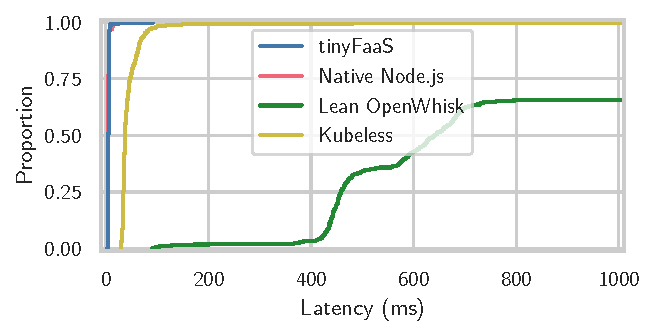
\includegraphics[width=\linewidth]{./fig/ecdf-pi-1.pdf}
        \caption{1 Thread}
        \label{fig:pigraph:1}
    \end{subfigure}
    \hfill
    \begin{subfigure}{0.49\linewidth}
        \centering
        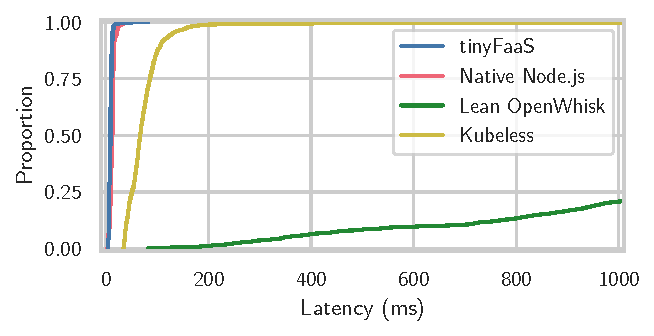
\includegraphics[width=\linewidth]{./fig/ecdf-pi-4.pdf}
        \caption{4 Threads}
        \label{fig:pigraph:4}
    \end{subfigure}
    \vfill
    \begin{subfigure}{0.49\linewidth}
        \centering
        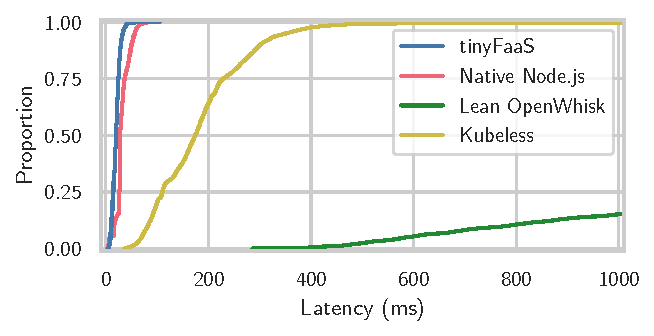
\includegraphics[width=\linewidth]{./fig/ecdf-pi-16.pdf}
        \caption{16 Threads}
        \label{fig:pigraph:16}
    \end{subfigure}
    \hfill
    \begin{subfigure}{0.49\linewidth}
        \centering
        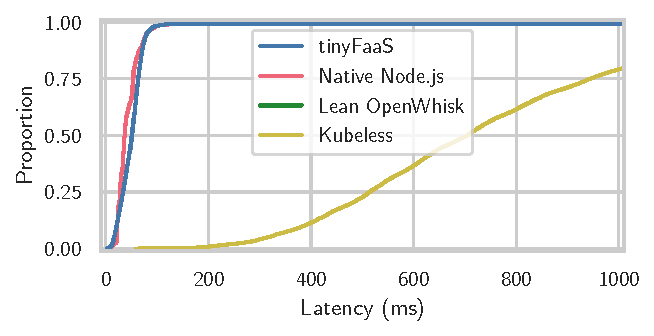
\includegraphics[width=\linewidth]{./fig/ecdf-pi-64.pdf}
        \caption{64 Threads}
        \label{fig:pigraph:64}
    \end{subfigure}
    \vfill
    \begin{subfigure}{0.49\linewidth}
        \centering
        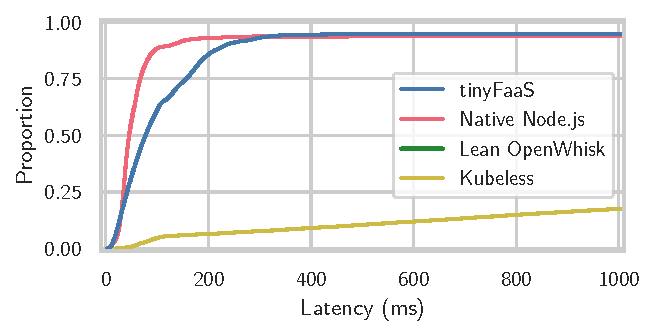
\includegraphics[width=\linewidth]{./fig/ecdf-pi-256.pdf}
        \caption{256 Threads}
        \label{fig:pigraph:256}
    \end{subfigure}
    \hfill
    \begin{subfigure}{0.49\linewidth}
        \centering
        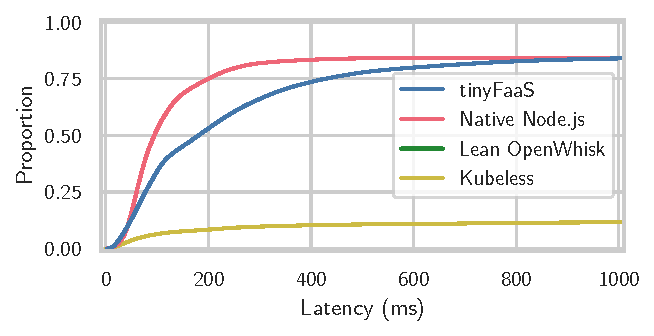
\includegraphics[width=\linewidth]{./fig/ecdf-pi-1024.pdf}
        \caption{1,024 Threads}
        \label{fig:pigraph:1024}
    \end{subfigure}
    \caption{Latency Measurements on Single-Board Computer}
    \label{fig:pigraph}
\end{figure}

\begin{figure}
    \begin{subfigure}{0.49\linewidth}
        \centering
        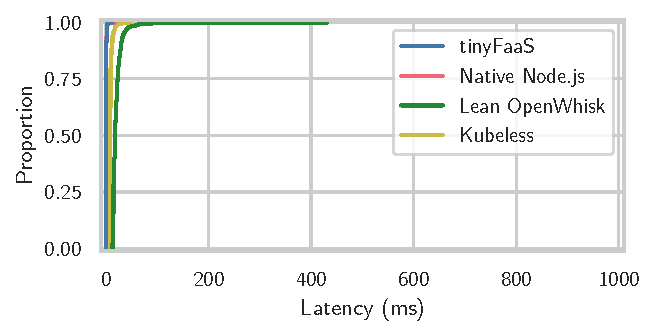
\includegraphics[width=\linewidth]{./fig/ecdf-aws-1.pdf}
        \caption{1 Thread}
        \label{fig:awsgraph:1}
    \end{subfigure}
    \hfill
    \begin{subfigure}{0.49\linewidth}
        \centering
        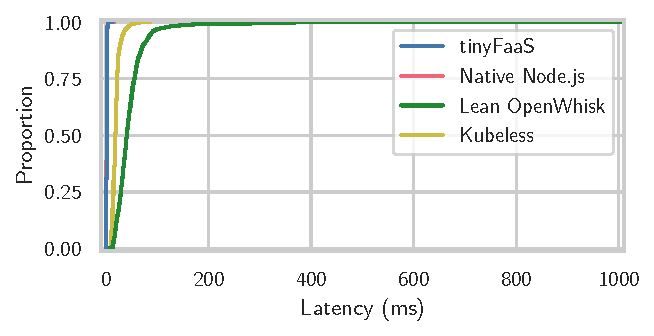
\includegraphics[width=\linewidth]{./fig/ecdf-aws-4.pdf}
        \caption{4 Threads}
        \label{fig:awsgraph:4}
    \end{subfigure}
    \vfill
    \begin{subfigure}{0.49\linewidth}
        \centering
        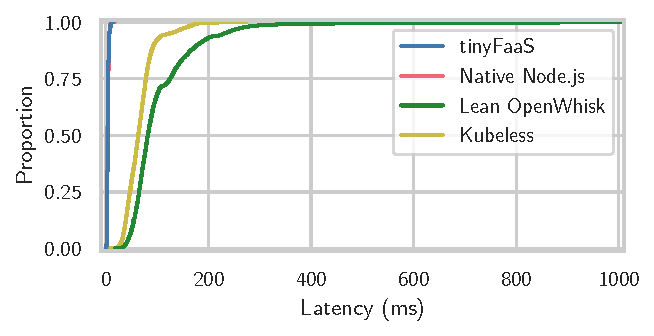
\includegraphics[width=\linewidth]{./fig/ecdf-aws-16.pdf}
        \caption{16 Threads}
        \label{fig:awsgraph:16}
    \end{subfigure}
    \hfill
    \begin{subfigure}{0.49\linewidth}
        \centering
        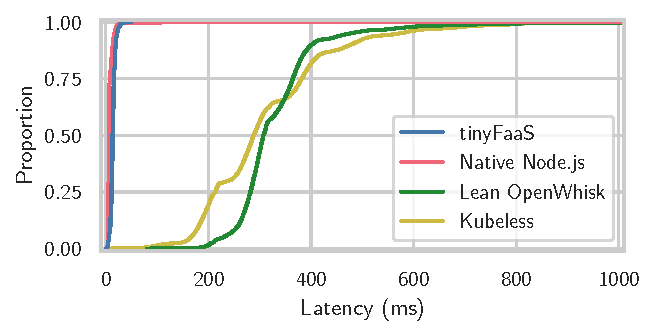
\includegraphics[width=\linewidth]{./fig/ecdf-aws-64.pdf}
        \caption{64 Threads}
        \label{fig:awsgraph:64}
    \end{subfigure}
    \vfill
    \begin{subfigure}{0.49\linewidth}
        \centering
        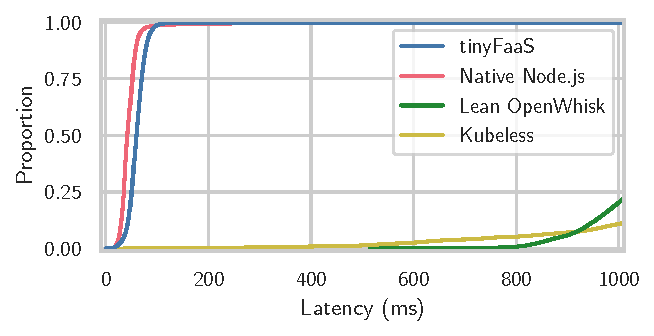
\includegraphics[width=\linewidth]{./fig/ecdf-aws-256.pdf}
        \caption{256 Threads}
        \label{fig:awsgraph:256}
    \end{subfigure}
    \hfill
    \begin{subfigure}{0.49\linewidth}
        \centering
        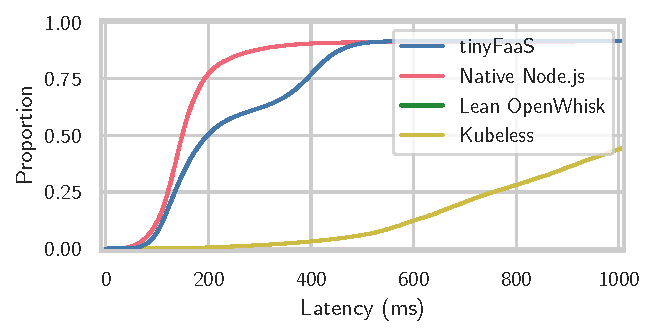
\includegraphics[width=\linewidth]{./fig/ecdf-aws-1024.pdf}
        \caption{1,024 Threads}
        \label{fig:awsgraph:1024}
    \end{subfigure}
    \caption{Latency Measurements on Cloud Server}
    \label{fig:awsgraph}
\end{figure}

In our experiments, we find that the best case average execution time for our exemplary function is 6ms on the single-board computer and 1ms on the cloud server.
These values are taken from the test against the native Node.js implementation using a low load of one parallel request.
For our results, we consider all operations that do not return any response and those with a response time of more than one second as failed.

\paragraph{Overhead of tinyFaaS}
\cref{fig:pigraph,fig:awsgraph} show the cumulative distribution of the respective latency measurements.
Please, note that this also shows the success rate for each experiment.
We show the measurements for \textit{tinyFaaS} along with each of the systems we compare it to, namely the native Node.js implementation, Lean OpenWhisk, and Kubeless.
As each client thread in our benchmarking tool only sends a new request when it receives a response or the previous request times out, throughput varies across all experiments.
We achieve the highest throughput of 9,800 operations per second with the native Node.js implementation on the Raspberry Pi with 1024 simultaneous connections.
On average, the benchmarking client issues a load of 38 operations per second per client thread on the Raspberry Pi and 172 operations per second per client thread on the cloud server.

\cref{fig:pigraph} shows that performance of \textit{tinyFaaS} is comparable to the native deployment on the Raspberry Pi.
Especially the success rates being equal shows that both scale equally well and that \textit{tinyFaaS} introduces a low to acceptable overhead.
At small scale both perform equally well in terms of response latency.
In fact, in our tests with 16 simultaneous client connections (\cref{fig:pigraph:16}), \textit{tinyFaaS} outperforms by 59\%.
We expect this to be caused by the implementation of CoAP in Node.js compared to our use of HTTP within our Node.js function handlers.
Furthermore, using multiple function handlers could help distribute load more evenly across CPU cores which Node.js by default does not do without explicitly designing for multithreading.
Nevertheless, for high loads the native implementation is about 40\% faster than \textit{tinyFaaS}.
As shown in \cref{fig:awsgraph}, results look similar in our cloud server experiments.
Unlike the single-board computer experiments, these do not show \textit{tinyFaaS} outperforming the native implementation at low load.
The reason for this might be that the cloud server has only two available CPU cores, albeit much more powerful ones, which could limit the impact of the multithreading advantage.
On average, the native implementation is 8\% faster than \textit{tinyFaaS} for small loads and 33\% faster with a medium to high load.

\paragraph*{tinyFaaS vs. Lean OpenWhisk}
Lean OpenWhisk on a constrained system as our Raspberry Pi is much slower than \textit{tinyFaaS} and scales considerably worse.
Even with just a single concurrent connection Lean OpenWhisk is unable to successfully respond to about two thirds of all requests.
In addition, the average latency for successful requests is almost 100 times as high as for \textit{tinyFaaS}.
With 256 and 1024 client threads (\cref{fig:awsgraph:256,fig:awsgraph:1024}), Lean OpenWhisk on our single-board computer fails completely with no successful response to any request.
In fact, we observed that the Raspberry Pi would not accept any more input at all and needed to be reset after each test.
We presume that the high memory usage of Lean OpenWhisk led to swapping which in turn put a high demand on the processor.
On the cloud server, results look slightly better for small to medium loads.
Lean OpenWhisk is able to successfully respond to all requests, albeit with a latency that is 20 times higher than that of \textit{tinyFaaS}.
Despite that, unlike \textit{tinyFaaS}, Lean OpenWhisk is not able to scale beyond 256 client threads.

\paragraph*{tinyFaaS vs. Kubeless}
Kubeless scales better than Lean OpenWhisk on the constrained Raspberry Pi but still has about 20\% error rate even under medium load.
At higher load levels, it also fails completely, i.e., does not return any results.
Response latency for Kubeless is better than Lean OpenWhisk, yet on average still more than eight times as high as the latency of \textit{tinyFaaS}.
We did expect Kubeless to be more powerful than Lean OpenWhisk based on~\cite{Palade2019-mo}, nonetheless Kubeless and Minikube do seem to introduce considerable overhead.
Furthermore, some part of that overhead can likely be attributed to the use of HTTP instead of the more efficient CoAP.
Results for the cloud server experiments appear comparable, except for Kubeless scaling up a bit further, which is expected given the more powerful hardware.
On average, Kubeless is 13 times slower than \textit{tinyFaaS} in these measurements.

These benchmark results reveal some important insights about the performance of \textit{tinyFaaS}.
Even though our proof-of-concept lacks more advanced features such as a more intelligent scheduling and container management, it was able to beat Lean OpenWhisk and Kubeless in throughput and scalability.
The performance difference is especially apparent when running these platforms on resource constrained hardware such as our Raspberry Pi.
As in an edge computing environment performance on constrained, single node devices is crucial, this shows that \textit{tinyFaaS} is the better fit for such environments.
